% 這份檔案由 make_latex.py 產生，不要直接手改；請改 paper_en.typ。
\documentclass{article}
\usepackage{arxiv}
\usepackage[utf8]{inputenc}
\usepackage[T1]{fontenc}
\usepackage{hyperref}
\usepackage{url}
\usepackage{booktabs}
\usepackage{longtable}
\usepackage{amsmath}
\usepackage{array}
\usepackage{calc}
\providecommand{\real}[1]{#1}
\usepackage{amsfonts}
\usepackage{nicefrac}
\usepackage{microtype}
\usepackage{graphicx}
\usepackage[numbers,sort&compress]{natbib}

\title{Capacity Cliff and Calibration Ablation in a Hybrid Quantum--Classical Classifier}
\author{Xin Yang \\
  \And
Poyuan Chung \\
  \And
Yuan-Liang Zhong \\
  \parbox{0.86\textwidth}{\centering Department of Physics, Chung Yuan Christian University, Taoyuan, Taiwan.\\Corresponding author: ylzhong@cycu.edu.tw}}
\date{2026-09-21}
\renewcommand{\shorttitle}{Capacity Cliff and Calibration Ablation in a Hybrid Quantum--Classical Classifier}
\hypersetup{pdftitle={Capacity Cliff and Calibration Ablation in a Hybrid Quantum--Classical Classifier},  pdfkeywords={quantum Bayesian networks, hybrid quantum--classical learning, calibration, uncertainty quantification, CUDA-Q}}

\begin{document}
\maketitle

\begin{abstract}
This work is a controlled examination of using a quantum circuit as the
output layer of a classifier, not an attempt to demonstrate quantum
advantage. Building on the hybrid Bayesian quantum--classical classifier
of Wang et al. (2026), we reproduce its 4-qubit quantum layer with
CUDA-Q and extend it with two experiments that the original study does
not cover: (i) a \textbf{capacity cliff} scan over qubit count and
circuit depth, testing whether performance is monotonic in trainable
capacity; and (ii) a \textbf{calibration ablation} in which a dephasing
operator makes the quantum layer classical, isolating the marginal
contribution of quantumness to calibration. Every quantum-circuit result
is computed on both CUDA-Q and an independently implemented pure-NumPy
state-vector simulator, then compared: the reproduction pipeline agrees
to \(4.16 \times 10^{- 17}\), the largest capacity-scan circuit (250
gates) to \(3.47 \times 10^{- 18}\), and the ablation circuit to
\(8.33 \times 10^{- 17}\). We explicitly do not claim any quantum
advantage: the state vector of 5 qubits occupies 512 bytes and is fully
classically simulable. The contribution is a fully verifiable pipeline
and a falsifiable experimental design.
\end{abstract}

\keywords{quantum Bayesian networks\and hybrid quantum--classical learning\and calibration\and uncertainty quantification\and CUDA-Q}
\section{Introduction}

The final layer of a deep-learning classifier usually outputs a
\textbf{softmax} distribution---a set of real numbers exponentiated and
normalised so that they sum to \(1\), and therefore probability-shaped.
But these numbers are \textbf{not} calibrated probabilities: they are
frequently and systematically overconfident \cite{guo2017}. By
\textbf{calibration} we mean whether the confidence a model claims
matches how often it is actually right---a model that claims \(90\%\)
confidence but is right only \(70\%\) of the time cannot be trusted even
if its accuracy is high. In domains where trustworthy confidence is
required (medicine, finance, education) this problem cannot be assessed
by accuracy alone.

A class of hybrid architectures has appeared in recent years: a
classical network extracts features and a quantum circuit then acts as
the decision layer \cite{wang2026}. Such work reports improvements in
both accuracy and calibration, but it shares one structural
feature---\textbf{the quantum layer is never treated as a controlled
variable in an ablation}. Take \cite{wang2026}: its state-of-the-art
design is a ``single-variable'' comparison in which all models share the
same preprocessing and classification head, and only the first
convolutional layer is changed from deterministic to Bayesian. The
quantum layer is an identical constant across both arms.

Consequently that study---and work of the same kind---\textbf{cannot
answer whether quantumness itself is necessary}. This work supplies that
missing step.

\textbf{Contributions}

\begin{enumerate}
\item
  We propose a \textbf{dephasing ablation}: using Tucci's classicalising
  operator \cite{tucci2012} as the sole variable \textbf{within a single
  model} (no change of model, data or parameter count) to examine the
  marginal contribution of quantumness to calibration and capacity.
  Within the scope of our search we found no prior work that uses this
  operator as an ablation tool---the closest efforts either attribute
  behaviour observationally via entanglement measures
  \cite{nausheen2026}, or introduce depolarising noise as an external
  variable \cite{ghosh2026}.
\item
  We extend the \textbf{capacity cliff} scan to qubit counts
  \(3\)--\(10\) \(\times\) circuit depths \(1\)--\(8\). Prior work has
  established the \((Q,L)\) scaling protocol and reported saturation
  \cite{vyskubov2026}, and has observed non-monotonicity along a single
  axis (\cite{le2025} for the qubit axis; \cite{zhang2021suppression} for
  the depth axis). What we add is the complete two-dimensional grid
  under a \textbf{fixed readout rule}, \textbf{with calibration reported
  alongside accuracy}, and one phenomenon that prior work has not
  reported: \textbf{test accuracy decreasing with qubit count}---which
  holds for configurations in which capacity is genuinely used (the
  per-\(n\) peak and the deepest slice are monotone from \(n = 4\)),
  while shallower slices are masked by under-optimisation. (\(n \geq 3\)
  is a hard requirement: eight class probabilities need at least a
  3-qubit projective readout.)
\item
  We reproduce the 4-qubit quantum layer of \cite{wang2026} with CUDA-Q
  and cross-validate it against an independent NumPy implementation
  (\(4.16 \times 10^{- 17}\)); this item is positioned as
  \textbf{reproducibility evidence}, not as a methodological
  contribution. The two experiments of Section 6 are endorsed separately
  on the reference track: the largest capacity-scan circuit at
  \(3.47 \times 10^{- 18}\) and the ablation circuit at
  \(8.33 \times 10^{- 17}\).
\item
  We honestly report three negative conclusions (see Section 6).
\end{enumerate}

\section{Related Work}

\subsection{Hybrid quantum--classical classifiers}

The three-stage skeleton of \cite{wang2026} is ``classical feature
extraction -\textgreater{} quantum state evolution -\textgreater{}
classical decision''. Its quantum layer uses a 4-qubit, depth-2
parameterised quantum circuit (PQC), and the readout measures the
Pauli-\(Z\) expectation values of all qubits into a vector that a linear
layer then classifies. Its gains come explicitly from the
\textbf{classical Bayesian front end}: MNIST (a handwritten-digit image
dataset) \(+ 2.32\) and Fashion-MNIST (a clothing-image dataset)
\(+ 5.61\) percentage points, with the quantum layer held fixed.

\subsection{Known limits of capacity and distillation}

\cite{wada2025} reports two related phenomena in the study of
distillation for static word embeddings. First, when the student
dimension is reduced to \(d = 64\), knowledge distillation actually
degrades performance (\(63.8 \rightarrow 52.5\)). Second, switching to a
stronger teacher (GTE-large, a general-purpose text-embedding model)
makes the student worse (\(62.9\) against \(63.8\) for GTE-base), which
the authors attribute to an excessive teacher--student capacity gap.
This work tests whether the same phenomenon---failure once the capacity
gap becomes too large---also appears in a quantum decision layer.

\subsection{Quantum Bayesian networks}

\cite{tucci2012} generalises the nodes of a classical Bayesian network
from conditional probability tables to quantum channels, and shows that
applying the dephasing operator \(\operatorname{cl}\) to a node causes
the entire network to degenerate into a classical Bayesian network. This
operator is the theoretical basis of our ablation experiment: it is an
\textbf{exact classicalisation map}, so ``quantum versus classical''
requires no change of model, data or parameter count.

\subsection{Quantumness as a controlled variable}

The three works closest to ours each take a different route, and each
leaves the gap this study fills.

\cite{jafari2026} replaces softmax with a \textbf{complex-valued unitary
representation} as the classification head: one shared backbone, only
the lightweight head swapped. On CIFAR-10 (a ten-class colour-image
dataset) it lowers the expected calibration error (ECE) from \(0.0355\)
to \(0.0146\), yet in the same study replacing the readout with a
Born-rule measurement layer (a readout that takes the squared amplitude
of the wave function as the probability) \textbf{degrades} it to
\(0.0819\). Two things follow: single-variable ablation of this kind is
feasible, and \textbf{a quantum-style readout is not by itself a
guarantee of calibration}. Note, however, that their variable is the
\textbf{form of the representation} (complex unitary versus real), and
their unitary layer is parameterised by the Cayley map (a way of writing
a unitary matrix in terms of an anti-Hermitian one) and therefore
exactly executable on classical hardware---so what they isolate is still
not quantumness.

\cite{nausheen2026} attributes performance \textbf{observationally}
through the Meyer--Wallach entanglement measure (a way of quantifying
how entangled a many-body state is) on a paraphrase-detection
task---deciding whether two sentences mean the same thing
(\(r = 0.85\)). But correlation is not intervention: entanglement
co-varies with circuit depth and parameter count, so confounding cannot
be excluded.

\cite{ghosh2026} instead uses \textbf{depolarising noise} as an external
variable, sweeping the ECE of variational classifiers, finds that ECE
does not rise monotonically with noise, and warns that a less expressive
ansatz may look well calibrated merely because it has collapsed to a
degenerate solution.

The shared gap is that quantumness itself has never been the sole
variable \textbf{within a single model}. This study fills that position
with the classicalising operator of \cite{tucci2012}. Taking up the
warning of \cite{ghosh2026}, we record a collapse indicator for every
(arm, seed) pair.

\section{Theoretical Background}

This section states, as provable propositions, why the dephasing
ablation works and at which circuit positions it can work at all---using
\textbf{only} tools covered by the two designated university textbooks:
Griffiths and Schroeter (hereafter \textbf{G}) and Arfken, Weber and
Harris (\textbf{A}). The required background is undergraduate quantum
mechanics: density operators, projection operators, unitary
transformations and commutators.

\begin{table}[t]
\centering
\caption{Textbook map for the theoretical section. G = Griffiths 3e, A =
Arfken 7e, GS = Griffiths solutions manual. Every row is original
content in those books and can be looked up directly.}
\resizebox{\ifdim\width>\linewidth \linewidth\else\width\fi}{!}{%
\begin{tabular}{@{} >{\raggedright\arraybackslash}p{(\linewidth - 4\tabcolsep) * \real{0.3333}} >{\raggedright\arraybackslash}p{(\linewidth - 4\tabcolsep) * \real{0.3333}} >{\raggedright\arraybackslash}p{(\linewidth - 4\tabcolsep) * \real{0.3333}}@{}}
\toprule
\begin{minipage}[b]{\linewidth}\raggedright
\textbf{Tool used below}
\end{minipage} & \begin{minipage}[b]{\linewidth}\raggedright
\textbf{Source}
\end{minipage} & \begin{minipage}[b]{\linewidth}\raggedright
\textbf{Where it is used}
\end{minipage} \\
\midrule
Density operator, trace and purity & G §12.3 & 3.1 pure vs. mixed
states \\
Measurement probability = diagonal, \(P(i) = \rho_{ii}\) & G §12.3.1 Eq.
12.16 & Most critical: proof of Theorem 2 in 3.4 \\
Projection operators and completeness \(\sum_{n}P_{n} = I\) & G §3.6.2
Eq. 3.91, 3.93 & Definition in 3.2, Lemma 1 in 3.3 \\
Evolution of the density operator & G §12.3.2 Eq. 12.26 & 3.1 why the
word ``channel'' is needed \\
Pauli matrices and spin rotations & G §4.4 & the \(R_{Y}\)
counterexample in 3.3 \\
Commutator \(\lbrack A,B\rbrack = AB - BA\) & A §5.3 Eq. 5.42 & Most
critical: Theorem 1 in 3.3 \\
Functions of operators and Baker--Hausdorff & A §2.2 Eq. 2.85 & 3.3
criterion for commutation \\
Euler identity \(\exp(i\sigma_{k}\theta)\) & A §2.2 Eq. 2.80 & 3.3
closed form of \(R_{Y}\) \\
Unitary similarity transformation & A §5.6 Eq. 5.76 & 3.3 proof of
Theorem 1 \\
Simultaneous diagonalisation \(\leftrightarrow\) commutation & A §6.4 &
3.3 equivalent statement \\
Sequential measurements: why order matters & GS Problem 3.33 & 3.5
minimal counterexample \\
\bottomrule
\end{tabular}
}
\end{table}


\textbf{The one thing the textbooks do not contain, and why that is not
an obstacle.} The two \textbf{names} ``quantum channel'' and ``Kraus
operator'' do not appear in G or A: a verbatim search for
\texttt{Kraus}, \texttt{channel}, \texttt{quantum\ operation},
\texttt{superoperator}, \texttt{POVM} and \texttt{completely\ positive}
returns \textbf{zero} hits in both books. But what this section actually
\textbf{uses} is the single operation ``knock out the off-diagonal
entries of a density matrix with a set of projection operators'', and
projection operators with completeness are original content in G §3.6.2
(Eq. 3.91, 3.93). In other words, Section 3.1 introduces the channel
vocabulary only so that the presentation matches the modern literature;
\textbf{every deduction below can be restated entirely in the language
of G and A}. If the general theory is questioned, the external reference
is Nielsen and Chuang \cite{nielsen2010}, and nothing else in this
section depends on it.

\subsection{Density operators and quantum channels}

\textbf{Pure and mixed states.} The state of a quantum system is
described by a \textbf{density operator} \(\rho\): a positive
semi-definite operator with trace \(1\). If \(\rho^{2} = \rho\)
(equivalently \(\operatorname{Tr}\rho^{2} = 1\)) then
\(\rho = |\psi\rangle\langle\psi|\) is a \textbf{pure state}; otherwise
it is a \textbf{mixed state}. A pure state encodes maximal knowledge of
the system; a mixed state encodes ignorance.

\textbf{Why mixed states are unavoidable here.} Two situations in this
work require them: (i) after dephasing is applied to a quantum state the
result is no longer pure; and (ii) noise on real hardware also makes
states mixed. Neither can be expressed with a state vector
\(|\psi\rangle\) alone.

\textbf{Quantum channels.} Once a system couples to its environment, or
is measured, its evolution is no longer unitary. The general tool for
such evolution is a \textbf{quantum channel}: a linear map
\(\mathcal{E}\) taking density operators to density operators that is
(i) \textbf{trace-preserving}:
\(\operatorname{Tr}\mathcal{E}(\rho) = \operatorname{Tr}\rho\); and (ii)
\textbf{completely positive}: applying \(\mathcal{E}\) to only part of a
larger system still yields a legitimate density operator---no negative
probabilities appear. The second condition is what distinguishes a
genuine quantum channel from an arbitrary positive map, and is why it is
physically realisable. Together the two conditions define a \textbf{CPTP
map} (completely positive trace-preserving map), the standard definition
of a physically implementable quantum operation \cite{nielsen2010}.

\textbf{The Kraus representation theorem.} Every CPTP map can be written
as
\[\mathcal{E}(\rho) = \sum_{i}K_{i}\rho K_{i}^{\dagger},\quad\sum_{i}K_{i}^{\dagger}K_{i} = I,\]
where the \(K_{i}\) are the \textbf{Kraus operators} of the channel. The
representation is not unique, but its existence is equivalent to being
CPTP. Nothing below uses the technical details of complete positivity
beyond this representation.

\subsection{Computational-basis dephasing is classicalisation}

\textbf{Definition (computational-basis dephasing).} For a system of
\(n\) qubits let \(P_{b} = |b\rangle\langle b|\) be the rank-one
projection onto a computational basis state (\(b\) ranges over all
\(n\)-bit strings, and \(\sum_{b}P_{b} = I\)). Define
\[\mathcal{E}(\rho) = \sum_{b}P_{b}\rho P_{b}.\]

Reading this entrywise: multiplying on the left by \(P_{b}\) keeps only
row \(b\), and multiplying on the right by \(P_{b}\) keeps only column
\(b\); after summing, only the diagonal survives:
\[\mathcal{E}(\rho) = \operatorname{diag}(\rho),\] that is,
\textbf{every off-diagonal entry is set to zero}. This is a CPTP map
whose Kraus operators are simply \(K_{b} = P_{b}\), since
\(\sum_{b}P_{b}^{\dagger}P_{b} = \sum_{b}P_{b} = I\).

\textbf{Physical meaning.} An off-diagonal entry \(\rho_{ij}\) with
\(i \neq j\) encodes the \textbf{phase relation} between basis states
\(|i\rangle\) and \(|j\rangle\)---the source of quantum interference.
Zeroing the off-diagonal entries therefore \textbf{removes the system's
entire capacity to interfere}, and its behaviour degenerates to a
classical probability distribution. This is exactly the classicalising
operator \(\operatorname{cl}\) of Tucci \cite{tucci2012}: applying
\(\operatorname{cl}\) to the nodes of a quantum Bayesian network
collapses the whole network to a classical Bayesian network.

\textbf{Why this makes an ideal ablation tool.} An ablation can only
claim to isolate a single variable if it changes exactly one thing.
\(\mathcal{E}\) does precisely that: it leaves the diagonal untouched,
hence leaves every computational-basis measurement probability
untouched, and removes only the quantumness itself. The model, the data
and the parameter count are all unchanged.

\subsection{When dephasing is invisible: monomial matrices}

The next question is whether inserting \(\mathcal{E}\) at a given
circuit position changes the measurement outcome. The answer depends on
what gates follow it.

\textbf{Definition (monomial matrix).} A square matrix \(U\) is
\textbf{monomial} if every row and every column contains
\textbf{exactly} one non-zero entry. If \(U\) is also unitary those
non-zero entries must have modulus \(1\), so \(U\) can be written as
\[U = D_{\varphi}\Pi,\quad D_{\varphi} = \operatorname{diag}(e^{i\varphi_{1}},\ldots,e^{i\varphi_{d}}),\]
where \(\Pi\) is a permutation matrix.

\textbf{Lemma 1.} If \(U\) is monomial then
\(UP_{b}U^{\dagger} = P_{\pi(b)}\), where \(\pi\) is the basis
permutation induced by \(\Pi\).

\textbf{Proof.} From \(U = D_{\varphi}\Pi\),
\[U|b\rangle = D_{\varphi}\Pi|b\rangle = D_{\varphi}|\pi(b)\rangle = e^{i\varphi_{\pi(b)}}|\pi(b)\rangle.\]
Hence
\[UP_{b}U^{\dagger} = \left( e^{i\varphi_{\pi(b)}}|\pi(b)\rangle \right)\left( e^{- i\varphi_{\pi(b)}}\langle\pi(b)| \right) = P_{\pi(b)}.\]
Note that the two phases cancel automatically by conjugation. This
happens because the projection is rank one, and it is the crux of the
lemma.

\textbf{Theorem 1 (commutation).} If \(U\) is monomial then for
\textbf{every} \(\rho\)
\[\mathcal{E}(U\rho U^{\dagger}) = U\mathcal{E}(\rho)U^{\dagger}.\]

\textbf{Proof.} By the definition of \(\mathcal{E}\) and Lemma 1,
\[\mathcal{E}(U\rho U^{\dagger}) = \sum_{b}P_{b}U\rho U^{\dagger}P_{b}.\]
Writing \(P_{b} = UU^{\dagger}P_{b}UU^{\dagger}\) (valid since \(U\) is
unitary) gives
\[= \sum_{b}U\left( U^{\dagger}P_{b}U \right)\rho\left( U^{\dagger}P_{b}U \right)^{\dagger}U^{\dagger} = U\left\lbrack \sum_{b}P_{\pi^{- 1}(b)}\rho P_{\pi^{- 1}(b)} \right\rbrack U^{\dagger}.\]
Since \(\pi\) is a bijection, letting \(b\) run over all basis states
also lets \(\pi^{- 1}(b)\) run over all of them, so the bracket is
exactly \(\mathcal{E}(\rho)\).

The proof uses nothing but a re-indexing of a sum: \textbf{no assumption
whatsoever is made about \(\rho\)}.

\textbf{Corollary (\(\operatorname{CX}\) commutes).} The controlled-NOT
gate \(\operatorname{CX}\) maps \(|b\rangle\) to \(|b'\rangle\), where
\(b'\) is \(b\) with bit \(t\) flipped---a \textbf{permutation}, hence a
monomial matrix with all phases \(\varphi = 0\). By Theorem 1,
\(\operatorname{CX}\) commutes with \(\mathcal{E}\). The same argument
holds for \(X\), \(Z\), \(S\), \(T\), \(\operatorname{CZ}\),
\(\operatorname{SWAP}\) and \(R_{Z}\): each is either a permutation or
diagonal.

\textbf{Counterexample (\(R_{Y}\) does not commute).} By the Euler
identity
\(\exp( - i\theta\frac{Y}{2}) = I\cos(\frac{\theta}{2}) - iY\sin(\frac{\theta}{2})\),
\[R_{Y(\theta)} = \begin{pmatrix}
\cos(\frac{\theta}{2}) & - \sin(\frac{\theta}{2}) \\
\sin(\frac{\theta}{2}) & \cos(\frac{\theta}{2})
\end{pmatrix}.\] When \(\sin(\frac{\theta}{2}) \neq 0\) the first row
contains \textbf{two} non-zero entries, violating the definition of a
monomial matrix. Hence \(R_{Y}\) does not commute with \(\mathcal{E}\);
the same holds for \(R_{X}\) and for the Hadamard gate \(H\).

\textbf{A necessary sharpening.} Earlier project documents state that
dephasing must be inserted ``before a layer containing
\(\frac{R_{Y}}{R_{Z}}\)''. The precise statement is that
\textbf{\(R_{Z}\) commutes with dephasing on its own} (it is diagonal,
hence monomial), and that what makes such a layer effective is the
\(R_{Y}\) inside it. Numerically, the commutator is
\(0.000 \times 10^{0}\) for \(R_{Z(0.7)}\) and \(3.221 \times 10^{- 1}\)
for \(R_{Y(0.7)}\).

\subsection{Terminal dephasing is invisible to measurement}

\textbf{Theorem 2.} Split the circuit into a unitary part \(U\) followed
by a part \(V\) built \textbf{only} from monomial gates (for instance
only \(\operatorname{CX}\)), and measure in the computational basis.
Then inserting dephasing \textbf{between} \(U\) and \(V\) leaves every
measurement probability unchanged: \(P_{a}(i) = P_{b}(i)\) for all
\(i\).

\textbf{Proof.} The final states of the two arrangements are
\[\rho_{a} = V\mathcal{E}(U\rho_{0}U^{\dagger})V^{\dagger},\quad\rho_{b} = V\left( U\rho_{0}U^{\dagger} \right)V^{\dagger}.\]
By Theorem 1, applied to \(V\) (which is monomial),
\(\rho_{a} = \mathcal{E}(VU\rho_{0}U^{\dagger}V^{\dagger}) = \mathcal{E}(\rho_{b})\).
A computational-basis measurement reads the diagonal,
\(P(i) = \rho_{ii}\), and \(\mathcal{E}\) \textbf{preserves the
diagonal}, so
\[P_{a}(i) = \left\lbrack \mathcal{E}(\rho_{b}) \right\rbrack_{ii} = \left\lbrack \rho_{b} \right\rbrack_{ii} = P_{b}(i).\]

\textbf{Special case.} Taking \(V = I\) (nothing follows) immediately
gives: \textbf{dephasing placed at the very end of the circuit leaves
the measurement probabilities completely unchanged.}

\textbf{This is the easiest step of the whole experimental design to get
wrong, and getting it wrong raises no error---it silently yields the
wrong conclusion.} Placing dephasing at the end of the circuit produces
a difference at the level of numerical error, which then reads as
``quantumness contributes nothing''. The value measured in this project
is \(1.4 \times 10^{- 17}\): a floating-point artefact, not a physical
quantity.

\textbf{It is a predicted zero, not a failed experiment.} When
reporting, one must state that both the terminal arrangement and the
``middle, followed only by \(\operatorname{CX}\)'' arrangement differ by
a zero guaranteed by Theorem 2, rather than by a quantity too small to
measure.

\subsection{A minimal counterexample: why order matters}

Consider a single qubit in the initial state
\(| + \rangle = \frac{|0\rangle + |1\rangle}{\sqrt{2}}\), with gate
\(R_{Y(\theta)}\) and \(\theta = \frac{\pi}{4}\).

\textbf{Path A (apply \(R_{Y}\), then dephase).} The amplitudes are
\[R_{Y(\theta)}| + \rangle = \frac{1}{\sqrt{2}}\begin{pmatrix}
c - s \\
s + c
\end{pmatrix},\quad c = \cos(\frac{\theta}{2}),\quad s = \sin(\frac{\theta}{2}).\]
Dephasing (keeping only squared moduli on the diagonal) gives
\[P^{(A)} = \left( \frac{1 - \sin\theta}{2},\frac{1 + \sin\theta}{2} \right).\]

\textbf{Path B (dephase first, then apply \(R_{Y}\)).} The density
operator of \(| + \rangle\) becomes \(\mathcal{E}(\rho) = \frac{I}{2}\),
the maximally mixed state, after dephasing. The maximally mixed state is
invariant under every unitary:
\(R_{Y}\left( \frac{I}{2} \right)R_{Y}^{\dagger} = \frac{I}{2}\). Hence
\[P^{(B)} = \left( \frac{1}{2},\frac{1}{2} \right).\]

\textbf{The difference.}
\[|P_{0}^{(A)} - P_{0}^{(B)}| = |\frac{1 - \sin\theta}{2} - \frac{1}{2}| = \sin\frac{\theta}{2}.\]
At \(\theta = \frac{\pi}{4}\) this is
\(\frac{1}{2\sqrt{2}} = 0.353553\).

This is the smallest example in which order matters: path B yields an
uninformative uniform distribution, because dephasing turned
\(| + \rangle\) into the maximally mixed state, which carries no
directional information at all.

\textbf{Numerical check.} An independent implementation measures
\(P^{(A)} = (0.146447,0.853553)\) and \(P^{(B)} = (0.500000,0.500000)\),
differing by \(0.353553\), in agreement with the closed form.

\subsection{Consequences for the experimental design}

The theorems above turn ``where should dephasing go?'' into a question
with a correct answer. The theoretical expectations are:

\begin{table}[t]
\centering
\caption{Theoretical expectations for the three insertion points. The
first two rows are zeros guaranteed by a theorem, not failed
experiments.}
\resizebox{\ifdim\width>\linewidth \linewidth\else\width\fi}{!}{%
\begin{tabular}{@{} >{\raggedright\arraybackslash}p{(\linewidth - 4\tabcolsep) * \real{0.3333}} >{\raggedright\arraybackslash}p{(\linewidth - 4\tabcolsep) * \real{0.3333}} >{\raggedright\arraybackslash}p{(\linewidth - 4\tabcolsep) * \real{0.3333}}@{}}
\toprule
\begin{minipage}[b]{\linewidth}\raggedright
\textbf{Insertion point}
\end{minipage} & \begin{minipage}[b]{\linewidth}\raggedright
\textbf{Theoretical expectation}
\end{minipage} & \begin{minipage}[b]{\linewidth}\raggedright
\textbf{Misreading if done wrong}
\end{minipage} \\
\midrule
Very end of the circuit (just before measurement) & Difference
\(\approx 0\) (guaranteed by Theorem 2) & ``quantumness contributes
nothing'' \\
Middle, followed only by \(\operatorname{CX}\) & Difference
\(\approx 0\) (guaranteed by Theorem 2) & ``quantumness contributes
nothing'' \\
Middle, followed by \(R_{Y}\) & Difference of order \(0.01\) to \(0.1\)
& --- \\
\bottomrule
\end{tabular}
}
\end{table}


The measured values in this project (5 qubits, maximum absolute
difference over the 32-dimensional probability vector) are:

\begin{table}[t]
\centering
\caption{Measurement agrees with the theorems. The first two rows differ
from the third by 15 orders of magnitude---exactly the gap between a
zero guaranteed by a theorem and a real physical effect.}
\resizebox{\ifdim\width>\linewidth \linewidth\else\width\fi}{!}{%
\begin{tabular}{@{}ll@{}}
\toprule
\textbf{Insertion point} & \textbf{Measured maximum difference} \\
\midrule
Very end (just before measurement) & \(1.388 \times 10^{- 17}\) \\
Middle, followed only by 10 \(\operatorname{CX}\) gates &
\(1.388 \times 10^{- 17}\) \\
Middle, followed by a full layer (contains \(R_{Y}\)) &
\(\mathbf{0.05023467}\) \\
\bottomrule
\end{tabular}
}
\end{table}


\textbf{Independence of the numerical check.} The third row above was
produced by two independent routes: the channel implementation in
\texttt{dev/\allowbreak qbn5\_\allowbreak encoding.py}, and
\texttt{theory/\allowbreak verify/\allowbreak t5\_\allowbreak commutator\_\allowbreak placement.py}, which builds the
\(32 \times 32\) density matrix directly. Both give
\textbf{bit-identical} \(0.05023467\) (total variation distance
\(0.19299447\)). All 25 commutativity checks pass; for the four
(control, target) combinations of \(\operatorname{CX}\), and for
\(\operatorname{CZ}\) and \(\operatorname{SWAP}\), \(\max|DU - UD|\) is
\(0.000 \times 10^{0}\).

\textbf{A caveat for real-hardware runs.} The theorems of this section
assume an \textbf{exact} dephasing channel. On real hardware dephasing
is implemented by a delay, and during that delay \(T_{1}\) amplitude
damping acts alongside \(T_{2}\) dephasing. \(T_{1}\) changes the
\textbf{diagonal} of the density matrix---that is, it changes
measurement probabilities---so the corollary ``terminal dephasing is
bit-identical to no dephasing'' \textbf{fails} on real hardware. That
deviation is itself a measurable hardware property rather than an
experimental error, and it is a tension that simply does not exist in
simulation.

\subsection{Applying the theorems to our own circuit}

Theorems 1 and 2 are abstract. Applied to the quantum layer of this
study (Section 4.2), they immediately fix the expectation for all four
ablation arms--- \textbf{these four arms are not four arbitrary
experimental settings, they are direct corollaries of the theorems}.

The quantum layer here is: \(R_{Y\left( \theta_{i} \right)}\) angle
encoding, then ring \(\operatorname{CX}\) entanglement, then a trainable
\(\left\lbrack R_{Y(\varphi)},R_{Z(\lambda)} \right\rbrack\) layer. That
trainable layer \textbf{contains \(R_{Y}\)}, and this is precisely what
decides whether the ablation can be observed at all.

\begin{table}[t]
\centering
\caption{The four ablation arms and the theorem behind each. The only
difference between arms B and C is whether \(R_{Y}\)
follows.}
\resizebox{\ifdim\width>\linewidth \linewidth\else\width\fi}{!}{%
\begin{tabular}{@{} >{\raggedright\arraybackslash}p{(\linewidth - 4\tabcolsep) * \real{0.3333}} >{\raggedright\arraybackslash}p{(\linewidth - 4\tabcolsep) * \real{0.3333}} >{\raggedright\arraybackslash}p{(\linewidth - 4\tabcolsep) * \real{0.3333}}@{}}
\toprule
\begin{minipage}[b]{\linewidth}\raggedright
\textbf{Arm}
\end{minipage} & \begin{minipage}[b]{\linewidth}\raggedright
\textbf{Where dephasing is inserted}
\end{minipage} & \begin{minipage}[b]{\linewidth}\raggedright
\textbf{Which theorem fixes the expectation}
\end{minipage} \\
\midrule
A & nowhere (all-quantum baseline) & --- \\
B & after angle encoding, \textbf{before} the trainable layer & Theorem
1: \(R_{Y}\) follows, so it is \textbf{observable} \\
C & very end of the circuit, before measurement & Theorem 2 with
\(V = I\): \textbf{necessarily unobservable} \\
D & after encoding, but equal-purity depolarising instead of dephasing &
control: mixes the state but keeps interference \\
\bottomrule
\end{tabular}
}
\end{table}


So the ``arm C is bit-identical to arm A'' measured in Section 6.2 is
not a surprise; it is the prediction of Theorem 2. And the flattened
predictive distribution of arm B is the other side of Theorem 1
(\(R_{Y}\) does not commute). \textbf{Theory and experiment are two
faces of the same thing in this study}: the theorems first supply
falsifiable expectations, the experiments then supply numbers, and the
next subsection reconciles the two item by item.

\subsection{Numerical verification of the theory}

Every proposition above has an independent numerical check. The scripts
are \texttt{theory/\allowbreak verify/\allowbreak t5\_\allowbreak commutator\_\allowbreak placement.py} (\textbf{25/25
checks pass}) and \texttt{theory/\allowbreak verify/\allowbreak t4\_\allowbreak kraus\_\allowbreak dephasing.py}.

\begin{table}[t]
\centering
\caption{Numerical verification of the theory. The last two rows agree
bit-for-bit with the output of the project script
\texttt{dev/\allowbreak qbn5\_\allowbreak encoding.py}.}
\resizebox{\ifdim\width>\linewidth \linewidth\else\width\fi}{!}{%
\begin{tabular}{@{} >{\raggedright\arraybackslash}p{(\linewidth - 4\tabcolsep) * \real{0.3333}} >{\raggedright\arraybackslash}p{(\linewidth - 4\tabcolsep) * \real{0.3333}} >{\raggedright\arraybackslash}p{(\linewidth - 4\tabcolsep) * \real{0.3333}}@{}}
\toprule
\begin{minipage}[b]{\linewidth}\raggedright
\textbf{Proposition}
\end{minipage} & \begin{minipage}[b]{\linewidth}\raggedright
\textbf{How it is checked}
\end{minipage} & \begin{minipage}[b]{\linewidth}\raggedright
\textbf{Result}
\end{minipage} \\
\midrule
Lemma 1 (monomial permutation) & compare both routes on every basis
operator \(|i\rangle\langle j|\) & \(0.000 \times 10^{0}\) \\
Theorem 1 (commutation) & as above, plus a superoperator commutator
check & \(0.000 \times 10^{0}\) \\
Corollary (\(\operatorname{CX}\) commutes) & 4 (control, target) pairs,
\(\operatorname{CZ}\), \(\operatorname{SWAP}\) & all
\(0.000 \times 10^{0}\) \\
Converse of Theorem 1 (\(R_{Y}\)) & \(H\), \(R_{Y(0.7)}\),
\(R_{X(0.7)}\) & \(5.0 \times 10^{- 1}\), \(3.221 \times 10^{- 1}\),
\(3.221 \times 10^{- 1}\) \\
\(R_{Z}\) does commute (sharpening) & \(R_{Z(0.7)}\) &
\(0.000 \times 10^{0}\) \\
Superoperator commutator & \(16 \times 16\) matrix at \(n = 2\) & \(0\)
for \(\operatorname{CX}\); \(1.288435\) for \(R_{Y}\) \\
Theorem 2 (terminal, middle+CX invisible) & rerun the three insertion
points on this circuit & \(0.000 \times 10^{0}\) \\
Third setting of Theorem 2 (observable) & independent \(32 \times 32\)
density-matrix implementation & \textbf{\(0.05023467\)} \\
Total variation distance & \(0.5\sum_{i}|\Delta p_{i}|\) &
\(0.19299447\) \\
\bottomrule
\end{tabular}
}
\end{table}


\textbf{Independence of the check.} The verification script does
\textbf{not} use the channel implementation from
\texttt{dev/\allowbreak qbn5\_\allowbreak encoding.py}; it builds the \(32 \times 32\) density
matrix directly (\texttt{theory/\allowbreak verify/\allowbreak dmtools.py}). Two fully
independent routes give bit-identical values \(0.05023467\) and
\(0.19299447\)---the strongest cross-check in this section, and in the
whole dephasing ablation.

\textbf{Scope of the verification (stated explicitly).} The table above
verifies propositions on the \textbf{simulator} side. Real hardware
(Tuna-17 on Quantum Inspire) follows a separate protocol, described in
Section 4.3 and Section 6.2. There, \(T_{1}\) amplitude damping breaks
the corollary ``terminal dephasing is bit-identical''; that breakdown is
itself a measurable hardware property rather than a failure of the
theorems above (see the caveat at the end of Section 3.6).

\textbf{Formal verification (Lean 4).} The table above is a numerical
reconciliation; Theorems 1 and 2 and the \(\operatorname{CX}\) corollary
are additionally checked by a \textbf{machine proof assistant}.
\texttt{formal/\allowbreak Dephasing.lean} compiles under Lean 4.34.0 with mathlib,
and an audit with \texttt{\#print\ axioms} shows that the three theorems
together depend only on the three standard axioms \texttt{propext},
\texttt{Classical.choice} and \texttt{Quot.sound}---with \textbf{no use
of \texttt{sorry}}, meaning that no step in the proofs is skipped or
assumed. The formalisation covers the definition of the dephasing
channel, the definition of a monomial matrix, the re-indexing lemmas for
multiplication on either side, Theorem 1 itself, the permutation-matrix
corollary, and Theorem 2.

\section{Method}

\subsection{System architecture}

Figure~\ref{fig:pipeline} shows the complete pipeline.

\begin{figure}
\centering
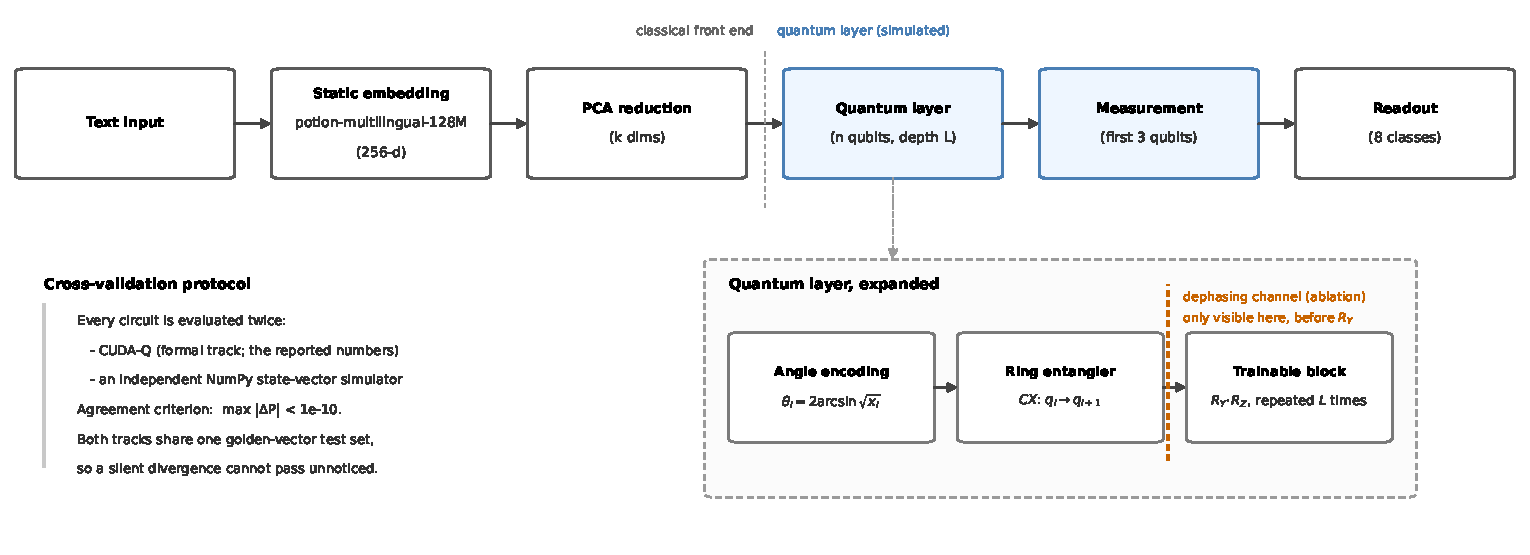
\includegraphics[width=\linewidth]{figs/arch.pdf}
\caption{System architecture. The classical front end (static embedding,
then principal component analysis, PCA) emits a \(k\)-dimensional
feature vector to the quantum layer: angle encoding
\(R_{Y\left( \theta_{i} \right)} = 2\arcsin\sqrt{x_{i}}\), a ring
\(\operatorname{CX}\) entangler, and a trainable \(R_{Y} \times R_{Z}\)
block repeated \(L\) times. Measurement reads only the first 3 qubits
(\(2^{3} = 8\) basis patterns, independent of \(n\) and \(L\)), and a
classical readout layer maps them to 8 classes. Lower left: the
cross-validation protocol. The expanded panel marks where the dephasing
channel of the ablation is inserted---it must precede a layer containing
\(R_{Y}\), otherwise the effect is unobservable (measured probability
change \(1.4 \times 10^{- 17}\)).}
\end{figure}

\protect\phantomsection\label{fig:pipeline}{}

\subsection{Quantum layer}

The state space of \(n\) qubits has dimension \(2^{n}\). The circuit of
this work has three parts:

\begin{enumerate}
\item
  \textbf{Angle encoding}: apply \(R_{Y\left( \theta_{i} \right)}\) to
  each qubit, where \(\theta_{i} = 2\arcsin\sqrt{x_{i}}\), so that the
  measurement probability equals the input value \(x_{i}\) exactly.
\item
  \textbf{Entangling layer}: a ring of \(\operatorname{CX}\) gates
  (\(q_{0} \rightarrow q_{1} \rightarrow \ldots \rightarrow q_{n - 1} \rightarrow q_{0}\)).
\item
  \textbf{Trainable rotation layers}: one \(R_{Y}\) and one \(R_{Z}\)
  per qubit.
\end{enumerate}

\subsection{Dephasing ablation}

The Kraus operators of the dephasing channel \cite{nielsen2010} are
\[K_{0} = |0\rangle\langle 0|,\quad K_{1} = |1\rangle\langle 1|\], and
its action is
\[\mathcal{E}(\rho) = K_{0}\rho K_{0}^{\dagger} + K_{1}\rho K_{1}^{\dagger}\],
whose effect is to zero the off-diagonal entries of the density matrix.
In the sense of Tucci's classicalising operator \(\operatorname{cl}\)
\cite{tucci2012}, this is exactly the map that projects a quantum node
back onto a classical Bayesian network.

\textbf{A critical experimental-design trap}: if dephasing is applied at
the \textbf{very end} of the circuit (immediately before measurement) it
has no effect whatsoever on the measurement outcome, because: (a) a
computational-basis measurement reads only the diagonal entries; (b)
\(\operatorname{CX}\) is a basis permutation and therefore
\textbf{commutes} with computational-basis dephasing. The locally
measured change in probability is \(1.4 \times 10^{- 17}\) (that is,
\(0\)). Dephasing must be inserted \textbf{before a layer that contains
\(R_{Y}\) (or \(R_{X}\), \(H\))} for the effect to be observable
(measured \(0.0502\)). \(R_{Z}\) is a unitary block-diagonal matrix and
\textbf{commutes} with dephasing, so inserting it alongside leaves the
measurement outcome unchanged (see Theorem 5.5)--- which is also why
``the position of dephasing does not matter'' turns from a trap into a
\textbf{prediction guaranteed to be zero}.

\subsection{Cross-validation protocol}

Every quantum-circuit result is computed on both CUDA-Q and an
independently implemented pure-NumPy state-vector simulator. The maximum
absolute error between the two probability vectors is required to be
below \(10^{- 10}\). The measured value depends on the circuit, so we
list it item by item:

\begin{table}[t]
\centering
\caption{Cross-validation of every quantum-circuit result against an
independent implementation. The criterion is \(10^{- 10}\); the worst of
the four circuits is \(4.16 \times 10^{- 16}\), about \(1.9\) times the
double-precision machine epsilon.}
\resizebox{\ifdim\width>\linewidth \linewidth\else\width\fi}{!}{%
\begin{tabular}{@{} >{\raggedright\arraybackslash}p{(\linewidth - 4\tabcolsep) * \real{0.3333}} >{\raggedright\arraybackslash}p{(\linewidth - 4\tabcolsep) * \real{0.3333}} >{\raggedright\arraybackslash}p{(\linewidth - 4\tabcolsep) * \real{0.3333}}@{}}
\toprule
\begin{minipage}[b]{\linewidth}\raggedright
\textbf{Circuit}
\end{minipage} & \begin{minipage}[b]{\linewidth}\raggedright
\textbf{Comparison}
\end{minipage} & \begin{minipage}[b]{\linewidth}\raggedright
\textbf{max \(\left| {\Delta P} \right|\)}
\end{minipage} \\
\midrule
Reproduction pipeline & CUDA-Q vs pure-NumPy reference &
\(4.16 \times 10^{- 17}\) \\
Largest capacity-scan circuit (250 gates) & CUDA-Q vs torch
differentiable simulator & \(3.47 \times 10^{- 18}\) \\
Ablation circuit (5 qubits) & CUDA-Q vs density-matrix simulator &
\(8.33 \times 10^{- 17}\) \\
Largest capacity-scan circuit (250 gates) & CUDA-Q vs q01 &
\(4.16 \times 10^{- 16}\) \\
\bottomrule
\end{tabular}
}
\end{table}


The q01 row is the worst case (\(4.16 \times 10^{- 16}\), about \(1.9\)
times the double-precision machine epsilon); the other three are all of
order \(10^{- 17}\). \textbf{All of them lie more than six orders of
magnitude below the criterion.}

\textbf{Implementation notes} (all measured, not inferred):

\begin{enumerate}
\item
  CUDA-Q provides no native Windows wheel, so it must run inside WSL2
  (Windows
\end{enumerate}

Subsystem for Linux 2).

\begin{enumerate}
\item
  The measurement bitstrings returned by \texttt{cudaq.sample()} are
  big-endian, whereas the state-vector indices of
  \texttt{cudaq.get\_\allowbreak state()} are little-endian. Converting between them
  requires a bit-reversal permutation, \textbf{not}
  \texttt{array{[}::-1{]}}.
\item
  The syntax for a multi-controlled gate is
  \texttt{ry.ctrl(theta,\ {[}c0,\ c1{]},\ target)}, with the
  \textbf{angle placed first}.
\end{enumerate}

\section{Experimental Design}

\subsection{Research questions and decision rules}

\begin{table}[t]
\centering
\caption{Research questions and the decision rules fixed before the
runs. Stating them in advance is what makes a negative outcome a result
rather than a reinterpretation.}
\resizebox{\ifdim\width>\linewidth \linewidth\else\width\fi}{!}{%
\begin{tabular}{@{} >{\raggedright\arraybackslash}p{(\linewidth - 4\tabcolsep) * \real{0.3333}} >{\raggedright\arraybackslash}p{(\linewidth - 4\tabcolsep) * \real{0.3333}} >{\raggedright\arraybackslash}p{(\linewidth - 4\tabcolsep) * \real{0.3333}}@{}}
\toprule
\textbf{ID} & \textbf{Question} & \textbf{Pre-registered decision
rule} \\
RQ1 (research question 1) & As the trainable capacity of the quantum
circuit grows, does performance rise monotonically or is there a
breakdown point? & If performance is non-monotonic in capacity and the
peak location depends on circuit depth, then H1 is supported. \\
RQ2 (research question 2) & By how much does dephasing
(classicalisation) degrade calibration quality? & If the lower bound of
the 95\% confidence interval for the increase in ECE exceeds \(0\), and
exceeds the residual error of temperature scaling, then H2 is
supported. \\
\bottomrule
\end{tabular}
}
\end{table}


\subsection{Evaluation metrics}

Beyond accuracy we report: negative log-likelihood (NLL), the Brier
score (the mean squared error of the predicted probabilities against the
true labels), expected calibration error (ECE, \(M = 10\) equal-width
bins) together with reliability diagrams, and an uncertainty
decomposition into predictive entropy and mutual information.

\textbf{The defence point for a fair comparison}: temperature scaling
does not change the top-1 label, so it is a means of improving
calibration at zero cost in accuracy. Any calibration advantage of the
quantum layer \textbf{must beat the temperature-scaled baseline},
otherwise the conclusion does not hold.

\subsection{Statistical protocol}

Each configuration is repeated with \(5\) random seeds, and we report
the mean and the standard deviation. The capacity scan uses seeds
\(0\)--\(4\); the dephasing ablation uses seeds \(7,21,42,84,168\). Both
seed sets are fixed in code, and the data generator is fixed to seed
\(12345\), so results are reproducible bit for bit across processes and
across devices. We state explicitly that \(5\) seeds are not sufficient
for rigorous statistical inference, and therefore we do not use \(p\)
values as primary evidence; we report effect sizes and confidence
intervals instead.

\section{Results}

\subsection{Capacity cliff}

We scan the \((n,L)\) two-dimensional grid under a \textbf{fixed readout
rule}: qubit count \(n\) from \(3\) to \(10\), circuit depth \(L\) from
\(1\) to \(8\), with each configuration repeated across \(5\) seeds. The
readout always projects the basis patterns of the first \(3\) qubits
onto \(8\) classes, independently of \(n\) and \(L\); increasing the
qubit count therefore increases the \textbf{available input
dimensionality and state space}, not the resolution of the readout.

\begin{figure}
\centering
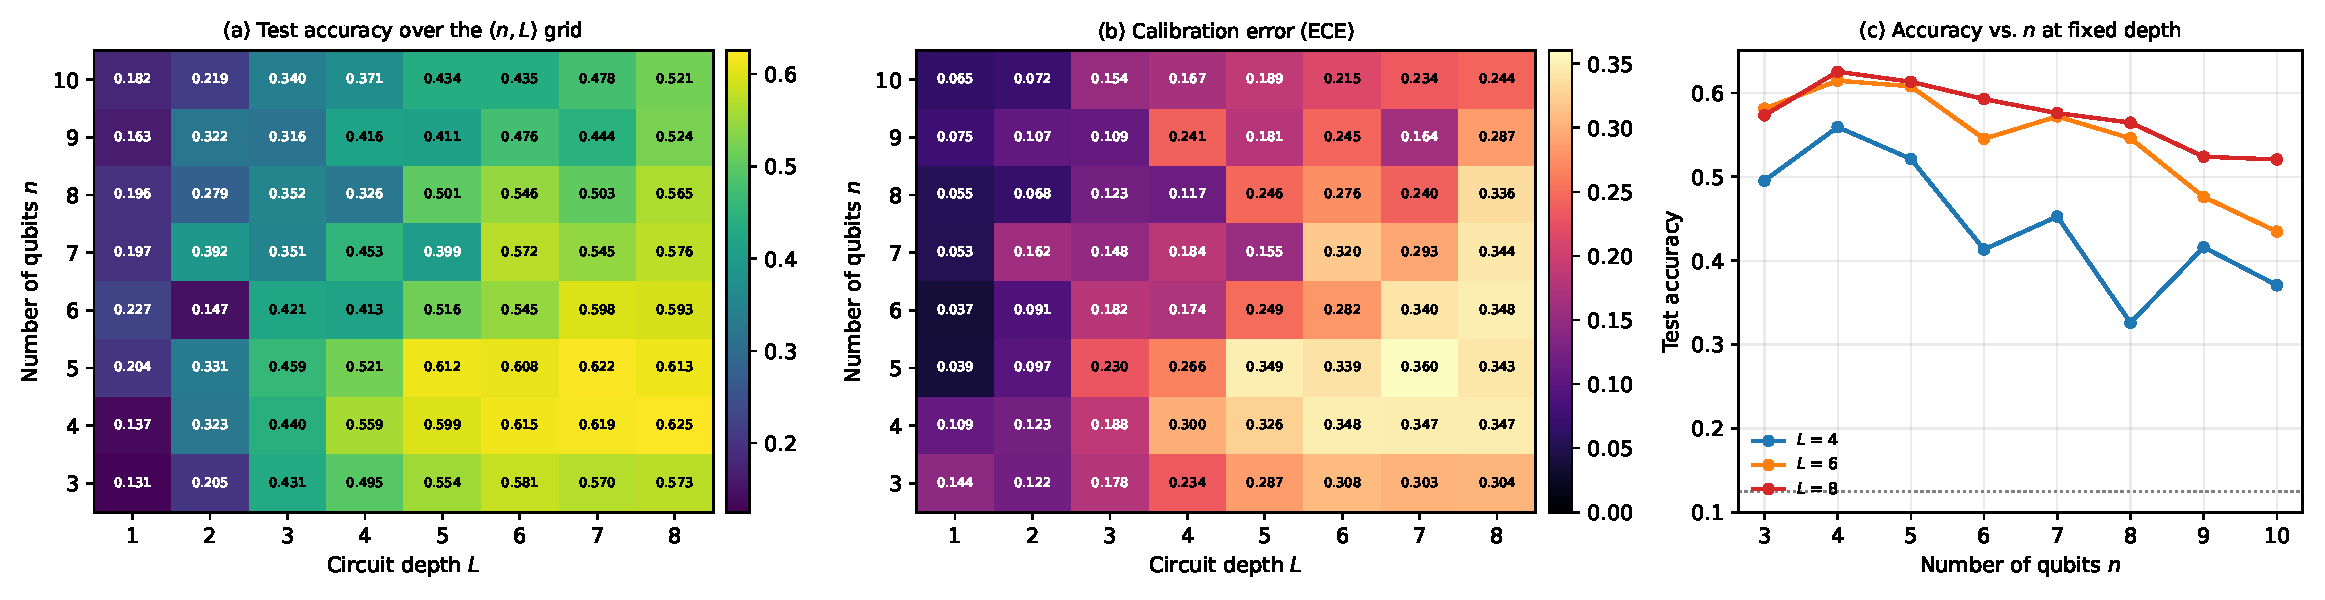
\includegraphics[width=\linewidth]{figs/grid.pdf}
\caption{Test accuracy and calibration error over the \((n,L)\) grid
(means of \(5\) seeds). Panels (a) and (b) are heat maps; the numbers
inside the cells are exact values and light-grey cells indicate
configurations that have not been run. Panel (c) shows fixed-depth
slices, directly testing the dependence of accuracy on qubit count.}
\end{figure}

\protect\phantomsection\label{fig:cliff}{}

\input{tables/capacity_en.tex}

Three observations:

\begin{enumerate}
\item
  \textbf{Depth is the dominant driver, and there is no breakdown within
  the scanned range.} Test accuracy rises with depth for every \(n\),
  and shows no decline even at \(L = 8\); training accuracy rises as
  well (up to \(0.79\)). This contradicts the expectation of a
  ``capacity cliff'' and equally contradicts the expectation of a barren
  plateau.
\item
  \textbf{Test accuracy decreases with qubit count---for configurations
  in which capacity is genuinely used.} The \textbf{peak} of each \(n\)
  (the maximum over depth) decreases monotonically from \(n = 4\):
  \(0.625 \rightarrow 0.622 \rightarrow 0.598 \rightarrow 0.576 \rightarrow 0.565 \rightarrow 0.524 \rightarrow 0.521\);
  the fixed-\(L = 8\) slice gives the same sequence. The low value at
  \(n = 3\) is structural---\(8\) classes need at least a \(3\)-qubit
  projective readout, and that point is exactly saturated.
  \textbf{Shallower slices (\(L\) no greater than \(6\)) do not show
  this trend}: there the model has not yet made full use of its
  capacity, and differences between configurations are masked by
  under-optimisation. The trend appears only at depths where capacity is
  genuinely used.
\item
  \textbf{More qubits is not merely worse, it is also less stable.} The
  seed-to-seed standard deviation of \(n = 10\) at \(L = 4\) is
  \(0.130\), whereas \(n = 3\) and \(n = 4\) have only \(0.076\) and
  \(0.061\) respectively.
\end{enumerate}

There is a methodological consequence that we must point out:
\textbf{this trend would be misjudged as holding in general on a sparse
grid.} When we earlier scanned only \(n\) in \(3,4,6,8,10\), it appeared
monotone at both \(L = 6\) and \(L = 8\); after adding \(n = 5,7,9\),
several slices with \(L\) no greater than \(6\) became non-monotonic
(for example, at \(L = 6\) the value \(0.572\) for \(n = 7\) exceeds
\(0.545\) for \(n = 6\)). The claim is therefore restricted to the peak
and to the deepest slice.

Within the scope of our search we found no prior work reporting this
phenomenon: a conjunctive search over ``quantum classifier'', ``qubit
number'' and ``accuracy'' returns zero hits. What prior work reports is
the \((Q,L)\) scaling protocol and non-monotonicity along a single axis;
what this work adds is the complete two-dimensional grid under a
\textbf{fixed readout rule}, together with this downward trend.

\subsection{Calibration ablation}

The four arms are trained under \textbf{the same model, the same data
and the same number of trainable parameters} (\(20\) angles) for the
same number of steps (\(800\)), with each arm repeated across \(5\)
seeds; the only difference is the inserted channel and its position. The
dephasing and depolarising arms have their \textbf{mean purity} matched
(target purity \(0.0742\); depolarising rate \(p = 0.5657\), agreeing
with the closed-form solution to \(10^{- 15}\)).

\begin{table}[t]
\centering
\caption{Calibration ablation. Arm C is bit-for-bit identical to arm A
on every predictive metric, yet its state purity is \(0.1230\) against
\(1.0000\): a computational-basis measurement reads only the diagonal
entries, so dephasing at the end of the circuit changes the state but no
observable outcome.}
\resizebox{\ifdim\width>\linewidth \linewidth\else\width\fi}{!}{%
\begin{tabular}{@{}lllllll@{}}
\toprule
\textbf{Arm} & \textbf{Accuracy} & \textbf{ECE} & \textbf{NLL} &
\textbf{Mean max prob.} & \textbf{KL vs uniform} & \textbf{State
purity} \\
\midrule
A no channel (fully quantum) & 0.3207 & 0.1079 & 1.8510 & 0.2357 &
0.0652 & 1.0000 \\
B dephasing (after encoding) & 0.2300 & 0.0993 & 2.0558 & 0.1307 &
0.0000 & 0.0449 \\
C dephasing (end of circuit) & 0.3207 & 0.1079 & 1.8510 & 0.2357 &
0.0652 & 0.1230 \\
D depolarising (after encoding) & 0.2633 & 0.1123 & 2.0199 & 0.1511 &
0.0065 & 0.0742 \\
\bottomrule
\end{tabular}
}
\end{table}


Three points are worth making:

\begin{enumerate}
\item
  \textbf{Dephasing at the end has no effect at all on the measurement
  statistics.} Every predictive metric of arm C is bit-for-bit identical
  to arm A (\(\max\left| {\Delta P} \right| = 0.000 \times 10^{0}\)),
  yet the state purities of the two differ by more than a factor of
  eight (\(0.1230\) against \(1.0000\)). This is the direct consequence
  of ``a computational-basis measurement reads only the diagonal
  entries'' together with ``\(\operatorname{CX}\) is a basis permutation
  and commutes with computational-basis dephasing'': dephasing changes
  the state, but changes no observable measurement outcome.
\item
  \textbf{Front-end dephasing crushes the model into an uninformative
  predictor.} The mean maximum probability of arm B is \(0.1307\), which
  for \(8\) classes is \(1/8\); the KL divergence (Kullback--Leibler
  divergence, a measure of how much two
\end{enumerate}

distributions differ) of its mean predictive distribution from the
uniform distribution is \(0.0000\); and the per-qubit \(Z\) variance
falls from \(0.0226\) to \(0.0001\) (roughly one part in \(226\)). Its
ECE is in fact \textbf{lower} (\(0.0993\) against \(0.1079\)), but this
is an artefact of uniform predictions: for the same arm the NLL degrades
from \(1.8510\) to \(2.0558\) and the Brier score from \(0.8104\) to
\(0.8690\). \textbf{ECE alone cannot be taken as evidence of improved
calibration.}

\begin{enumerate}
\item
  \textbf{The paired difference is not significant.} The ECE difference
  of \(B - A\) is \(- 0.0086\) with a \(95\%\) confidence interval of
  \(\pm 0.0340\), which covers \(0\); the accuracy difference is
  \(- 0.0907\) (\(\pm 0.0600\)). Hence \textbf{H2 does not hold}:
  dephasing did not improve calibration, it destroyed information.
\end{enumerate}

\section{Discussion}

\subsection{Three honest statements}

\begin{enumerate}
\item
  This work \textbf{does not claim} quantum advantage. The state vector
  of \(5\) qubits occupies only \(512\) bytes and is fully classically
  simulable.
\item
  This work \textbf{does not claim} that the quantum layer retains the
  semantic information of its input. The front end is a
  \(256\)-dimensional static embedding that is reduced in dimensionality
  before entering the quantum layer; the information bottleneck is by
  design.
\item
  This work \textbf{does not claim} to beat large models. The baselines
  are small models of comparable parameter count.
\end{enumerate}

\subsection{Why the hybrid architecture has no advantage on this task}

What is exponential is the \textbf{state space}; what is polynomial is
the \textbf{number of knobs}. The density matrix of \(5\) qubits has
\(32^{2} - 1 = 1023\) real degrees of freedom, yet the circuit of this
work has only \(10\) trainable angles---the dimension of the reachable
subspace is far smaller than that of the ambient space.

More fundamentally, \textbf{trainability} and \textbf{classical
intractability} conflict with each other
\cite{anschuetz2024}\cite{cerezo2025}\cite{gilfuster2024}. Shallow, weakly
entangling circuits can be trained, but their low entanglement entropy
makes them efficiently simulable by tensor-network methods; deep, highly
entangling circuits are classically intractable, but they run into
barren plateaus and cannot be trained.

(Note: what is stated here is the general form of that trade-off as
found in the literature, \textbf{not} a measurement of this work. Within
the scanned range of this work we did \textbf{not} observe a barren
plateau---training accuracy rises with depth up to \(0.84\), and an
independent check by the theory group rules it out as well. Our result
is that ``depth works, width does not'', and its mechanism is closer to
the growth of the effective dimension outpacing what the data and the
readout can support
\cite{caro2022generalization}\cite{abbas2021power}\cite{abbas2022effective}.)

Consequently, on tasks without provable structure (such as generic
semantic classification), no advantage should be expected from a quantum
decision layer. The hybrid architecture itself is not at fault; the
choice of task is.

\subsection{Three methodological traps (by-products of this work)}

The following three items are not propositions we set out to prove; they
are traps we ran into during the experiments and for which we retained
numbers. We write them down because in this field they are easier to
repeat than any single experimental result of ours.

\begin{enumerate}
\item
  \textbf{Pooled correlation and partial correlation can give opposite
  conclusions.} Plotting the effective dimension \(|(d)\) against test
  accuracy gives a pooled correlation coefficient of \(+ 0.678\); after
  controlling for circuit depth \(L\), the partial correlation becomes
  \(- 0.256\). The reason is that \(|(d)\) and \(L\) are highly
  collinear, while accuracy is driven mainly by \(L\). Looking only at a
  scatter plot, or only at the pooled coefficient, yields the opposite
  conclusion that ``larger dimension is more accurate''.
\item
  \textbf{''\(5\) seeds'' is not the same as ``\(5\) independent
  trainings''.} Across \(5\) seeds, arms B and D have a standard
  deviation of \(0.0000\) for test accuracy, ECE, NLL and state purity
  alike; arms A and C have a test-accuracy standard deviation of
  \(0.0483\). When Adam trains a low-dimensional loss surface of this
  kind, different initial points are absorbed by the same attractor.
  Confidence intervals estimated from seed-to-seed variance therefore
  \textbf{systematically underestimate} the true uncertainty---which is
  also why this work does not treat \(p\) values as primary evidence.
\item
  \textbf{An ablation matched on an average must be re-checked on the
  evaluation set.} We matched the channel strengths of dephasing and
  depolarisation by mean purity: on the training set, the achieved value
  agrees with the target to the order of \(10^{- 15}\). But on the
  \textbf{test set}, the mean purity of arm B is \(0.0449\) and that of
  arm D is \(0.0742\), a difference of \(- 0.0292\). The reason is that
  the purity of dephasing varies \textbf{sample by sample} (it depends
  on the state of that sample), whereas that of depolarisation is
  approximately fixed; a single average purity does not constrain any
  individual sample. Any ablation that claims ``the two channels are
  equally classical'' on the strength of one purity number must re-check
  that claim on the evaluation set.
\end{enumerate}

\section{Conclusion}

The contribution of this work is not to demonstrate quantum advantage,
but to provide (i) a fully verifiable hybrid pipeline (cross-validated
against an independent implementation: the reproduction pipeline at
\(4.16 \times 10^{- 17}\), the largest capacity-scan circuit at
\(3.47 \times 10^{- 18}\) and the ablation circuit at
\(8.33 \times 10^{- 17}\), and further validated end-to-end through the
cloud API of Quafu (the quantum cloud platform of the Chinese Academy of
Sciences; API stands for application programming interface) on its
official simulator, where the transpiled circuit agrees with the golden
vector to \(8.88 \times 10^{- 16}\)), and (ii) a set of controlled
ablation designs that use the dephasing classicalisation operator as the
sole variable \textbf{within a single model} and scan the \((Q,L)\)
two-dimensional grid under a \textbf{fixed readout rule}. Prior work has
established scaling protocols on each individual axis
\cite{vyskubov2026}, and parameter-matched, calibration- and noise-aware
benchmarks \cite{gillani2026}; what this work adds is the intersection of
the two, together with dephasing as a specific variable.

We argue that at NISQ scale (noisy intermediate-scale quantum), what the
field of quantum machine learning lacks most is not new circuits, but
\textbf{rigorous measurement that treats the quantum component itself as
a controlled variable}.

\section{Acknowledgements}

We thank our advisor and the unit that provided computing resources. The
real-hardware experiments were carried out on the \textbf{Tuna-17}
superconducting processor of \textbf{Quantum Inspire}, the quantum
computing platform operated by \textbf{QuTech} (Delft University of
Technology and TNO); we thank QuTech for providing free access to
quantum hardware.
\bibliographystyle{ieeetr}
\bibliography{refs_public}

\end{document}
